\documentclass{article}

\usepackage{amsmath}
\usepackage{amssymb}
\usepackage{amsthm}
\usepackage{authblk}
\usepackage[english]{babel}
\usepackage{blkarray}
\usepackage[font=small]{caption}
\usepackage{cite}
\usepackage{graphicx}

% ---- Author affiliations ---- %

\renewcommand\Affilfont{\itshape\small}

% ---- Propositions, lemmas, defintions... ---- %

\newtheorem{algorithm}{Algorithm}
\newtheorem{corollary}{Corollary}
\newtheorem{definition}{Definition}
%\newtheorem{example}{Example}
\newtheorem{lemma}{Lemma}
\newtheorem{proposition}{Proposition}
%\newtheorem{remark}{Remark}


% ---- Special environments (examples and remarks) ---- %

\newcounter{examplecounter}
\newenvironment{example}
{\small\vspace{0.5\baselineskip}
  \refstepcounter{examplecounter}%
  \noindent\textbf{Example \arabic{examplecounter}.}%
}{\vspace{-0.2\baselineskip}\begin{center}%
  $\star$\end{center}\vspace{0.5\baselineskip}}

\newcounter{remarkcounter}
\newenvironment{remark}
{\small\it\vspace{0.5\baselineskip}
  \refstepcounter{remarkcounter}%
  \noindent\textbf{Remark \arabic{remarkcounter}.}%
}{\vspace{0.5\baselineskip}}

\newenvironment{inset}
{\vspace{0.5\baselineskip}\begin{center}}
{\end{center}\vspace{0.5\baselineskip}}


% ---- Macros ---- %

\newcommand{\DN}{\scriptstyle{\Downarrow}}
\newcommand{\dn}{\scriptstyle{\downarrow}}
\newcommand{\up}[1]{\scriptstyle{(\uparrow)_{#1}}}
\newcommand{\eq}[1]{\scriptstyle{(\sim)_{#1}}}

\newcommand{\upg}{\scriptstyle{\uparrow}}
\newcommand{\eqg}{\scriptstyle{\sim}}

%---------------------------------------------------------------

\title{Calibrating MEM seeding heuristics}

\author[1,2]{Guillaume J. Filion}
\affil[1]{Genome Architecture, Gene Regulation, Stem Cells and Cancer
Programme, Center for Genomic Regulation (CRG), The Barcelona Institute of
Science and Technology, Dr. Aiguader 88, Barcelona 08003, Spain.}
\affil[2]{University Pompeu Fabra, Doctor Aiguader, 08003 Barcelona,
Spain.}

\date{\today}

%---------------------------------------------------------------
%---------------------------------------------------------------


\begin{document}

\maketitle

\begin{abstract}
The abstract will come later.
\end{abstract}


%---------------------------------------------------------------
%---------------------------------------------------------------

\section{Introduction}
Some introduction

\section{MEM seeds}

We can describe reads as sequences of four possible symbols representing
the state of the local match with the genome. The first symbol,
represented by a black square indicates a sequencing error. This is a
mismatch between the read and the genome so the nucleotide cannot belong
to a correct MEM seed. It either belongs to an incorrect MEM seed, or it
marks the end of a correct MEM seed.

The second symbol, represented by a black square with a white cross
indicates a sequencing error that is also a mismatch for \emph{all} the
duplicates. The nucleotide cannot belong to any MEM seed (correct or not)
so the next MEM seed must start at the following nucleotide. The symbol
`resets' the seeding process, which becomes in the same state as at the
beginning of the read.

The third symbol, represented by an exclamation mark indicates that the
target sequence is the only local match between the read and the genome.
This means that there is at least one mismatch between the read and any
duplicate since the beginning of the current MEM. From that nucleotide,
the MEM will extend forward until the next sequencing error. This means
that two exclamation marks must be separated by either a black square or a
black square with a cross.

The last symbol, represented as a white square indicates all the other
situations. This can mark the beginning but not the end of a MEM.

\section{Some definitions etc.}

\begin{figure}[h]
\centering
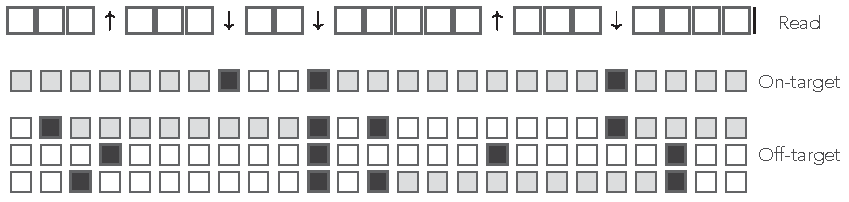
\includegraphics[scale=.9]{sketch_MEM.pdf}
\caption{\textbf{Reads and MEM seeds}. 
Some legend.}
\label{fig:sketch_MEM}
\end{figure}


We assume that the target sequence has $N$ duplicates that are potential
false positives for the seeding process. We further assume that
duplication was instantaenous and that all $N+1$ sequences diverge
independently from each other at a constant rate. In other words, we
ignore the complications due to the genealogy of the duplication events
and we simply assume that at each position, the target and a duplicate are
identical with probability $1-\mu$. In case they are not, we assume that
the duplicate has any of the remaining three nucleotides with equal
probability.

Each of the $N+1$ sequences of interest corresponds to a Bernoulli process
where `success' stands for a match between the sequence and the read, and
`failure' stands for a mismatch. To describe those processes, we will use
the `match function' $\varphi(n)$ that gives the length of the success
streak at position $n$. The processes are indexed such that $\varphi_0$
describes the matches of the target sequence, whereas $\varphi_j$ $(1 \leq
j \leq N)$ describes the matches of the duplicates. For instance,
$\varphi_0(5) = 5$ and $\varphi_1(5) = 3$ in the example of
Fig.~\ref{fig:sketch_MEM}.

For simplicity, we will refer to the Bernoulli processes as `threads', and
we will distinguish the `target thread' from the `duplicate threads'. At
any position $n$ of the read, a duplicate thread $j$ $(1 \leq j \leq N)$
is said to be `strictly masking' if $\varphi_j(n) > \varphi_0(n)$,
`potentially masking' if $\varphi_j(n) \geq \varphi_0(n)$ and
`non-masking' if $\varphi_j(n) < \varphi_0(n)$. There can be no MEM seed
at positions where there is a stricly masking thread. At positions where
there is a potentially masking thread any MEM seed must be a shared MEM
seed.


With these definitions, the decision tree for choosing the next symbol to
insert in a read can be summarized as in Fig.~\ref{fig:decision_tree}.
This sketch will be useful as a reference to compute the probabilities of
the blocks and their weighted generating functions.


\begin{figure}[h]
\centering
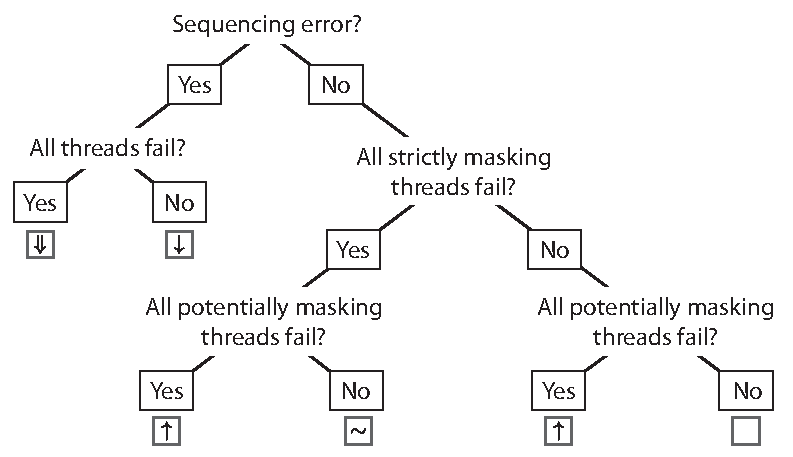
\includegraphics[scale=.7]{decision_tree.pdf}
\caption{\textbf{Decision tree}. 
Some legend.}
\label{fig:decision_tree}
\end{figure}



\begin{equation*}
\begin{blockarray}{ccccccccc}
   & \dn & \DN &\eq{1} & \ldots & \eq{\gamma-1} &
    \up{1} & \ldots & \up{\gamma-1} \\
\begin{block}{c[cccccccc]}
\dn & * & * & * & \ldots & * & * & \ldots & * \\
\DN & \tilde{A}_\infty(z) & \tilde{B}_\gamma(z) & 0 & \ldots & 0 &
    r_1(z) & \ldots & r_{\gamma-1}(z) \\
\eq{1} & * & * & 0 & \ldots & 0 & 0 & \ldots & G_{1,\gamma-1}(z) \\
\eq{2} & * & * & 0 & \ldots & 0 & 0 & \ldots & G_{2,\gamma-1}(z) \\
\vdots & \vdots & \vdots & \vdots & \ddots & \vdots & \vdots &
    \ddots & \vdots \\
\eq{\gamma-1} & * & * & 0 & \ldots & 0 & 0 & \ldots & 0 \\
\up{1} & A_{\gamma-1}(z) & B_{\gamma-1}(z) & 0 & \ldots & 0 & 0 &
    \ldots & 0 \\
\up{2} & A_{\gamma-2}(z) & B_{\gamma-2}(z) & 0 & \ldots & 0 & 0 &
    \ldots & 0  \\
\vdots & \vdots & \vdots & \vdots & \ddots & \vdots & \vdots &
    \ddots & \vdots \\
\up{\gamma-1} & A_1(z) & B_1(z) & 0 & \ldots & 0 & 0 & \ldots & 0 \\
\end{block}
\end{blockarray}.
\end{equation*}


\begin{definition}
The main thread is dominant at nucleotide $n$ if $\varphi_0(n) >
\varphi_i(n)$ for all $i$ $(1 \leq i \leq N)$. The main thread is
co-dominant if inequality is not strict and there exists $i$ $(1\leq i
\leq N)$ such that $\varphi_0(n) = \varphi_i(n)$.
\end{definition}

\subsection{Head vector}

At the beginning of the read, the match lengths of all the threads are
$0$. This is exactly the same as on a $\Downarrow$ symbol. We can thus
consider that the read starts in the $\Downarrow$ state, which is
equivalent to adding an edge labelled with the empty object $\varepsilon$
between the head vertex and the $\Downarrow$ vertex. The head vector is
thus
\begin{equation}
H(z) = (1,0, \ldots, 0).
\end{equation}


\subsection{Transitions from $\uparrow$}
\label{sec:trans_from_up}

After a $\uparrow$ symbol, the main thread becomes dominant. It will
remain so until the first read error, which can be a mismatch for all the
threads ($\Downarrow$ symbol), or for only some of them ($\downarrow$
symbol).

Since the read has no MEM seed, the $\Downarrow$ symbol or the
$\downarrow$ symbol must come before $\varphi_0(n) \geq \gamma$, which
imposes a limit on the number of $\square$ symbols that can follow a
$\square$ symbol. If nucleotide at position $n$ is the $\uparrow$ symbol
and $\varphi_0(n) = j$ $(1 \leq j \leq \gamma-1)$, the state of the read
is represented as $(\uparrow)_j$, meaning that the maximum number of
$\square$ symbols that can follow is $\gamma-1-j$.

Whether the nucleotides match the alternative threads is irrelevant until
the end of the block. The $\square$ symbols only mean that the nucleotides
are not error so their weighted generating function is $qz$. The
$\Downarrow$ symbol indicates an error -- probability $p$ -- that is also
a mismatch for the $N$ alternative threads -- probability $(1-\mu/3)^N$ --
so its weighted generating function is $pz(1-\mu/3)^N$. Likewise, the
weighted generating function of the $\downarrow$ symbol is seen to be
$pz(1-(1-\mu/3)^N)$.

The weighted generating function of the transition from $(\uparrow)_j$ to
$\Downarrow$ is
\begin{equation}
B_{\gamma-j}(z) = pz (1-\mu/3)^N \sum_{n=0}^{\gamma-j-1} (qz)^n.
\end{equation}

And the weighted generating function of the transition from
$(\uparrow)_j$ to $\downarrow$ is
\begin{equation}
A_{\gamma-j}(z) = pz (1-(1-\mu/3)^N) \sum_{n=0}^{\gamma-j-1} (qz)^n.
\end{equation}



\subsection{Transitions from $\Downarrow$}
\label{sec:trans_from_Down}

At a $\Downarrow$ symbol, all the threads have match length $0$ and the
read is `reset' to its initial state. The main thread is co-dominant with
all the alternative threads. The next terminator symbol depends on what
happens first. If all the alternative threads fail before the main thread,
the latter becomes dominant ($\uparrow$ symbol). If not all alternative
threads have failed when the main thread does, we need to distinguish two
cases: if all threads fail together with the main thread, the read is
reset ($\Downarrow$ symbol), otherwise the main read becomes dominated
($\downarrow$ symbol).

If the next terminator is the $\uparrow$ symbol, we need to distinguish
the cases based on the value of $\varphi_0$ (see
section~\ref{sec:trans_from_up}), which is just the position of
the $\uparrow$ symbol after the $\Downarrow$ symbol in this case. A
transition from $\Downarrow$ to $(\uparrow)_j$ consists of a succession of
$j$ correct nucleotides -- each with probability $q$. But we must also
make sure that no other $\uparrow$ symbol is inserted before position $j$.
We thus introduce $\xi_j$, the probability that at least one of the $N$
alternative threads survives at position $j$ after the $\Downarrow$ symbol. At
any correct nucleotide, the probability of failure of an alternative thread is
$\mu$, so
\begin{equation}
\xi_j = 1-(1-(1-\mu)^j)^N.
\end{equation}

The probablity of transition from $\Downarrow$ to $(\uparrow)_j$ is thus
$(\xi_{j-1}-\xi_j)q^j$ and the associated weighted generating function is
\begin{equation}
r_j(z) = (\xi_{j-1}-\xi_j)(qz)^j.
\end{equation}

If the next terminator is $\downarrow$, there is no limit on the number of
$\square$ symbols that can be inserted. Indeed, the main thread will not
be part of the MEM in this case. As mentioned in
section~\ref{sec:trans_from_up}, the weighted generating function of the
$\downarrow$ symbol is $pz(1-(1-\mu/3)^N)$. The probability that it first
occurs at position $n+1$ after the $\Downarrow$ symbol is the probability
that the first $n$ nucleotides are correct -- each with probability $q$
-- and that at least one alternative thread survives -- probability
$\xi_n$. The weighted generating function of the transition from
$\Downarrow$ to $\downarrow$ is thus
\begin{equation}
\tilde{A}_\infty(z) = pz(1-(1-\mu/3)^N)
  \sum_{n=0}^\infty \xi_n \cdot (qz)^n.
\end{equation}


Finally, if the next terminator is $\Downarrow$, there is a limit on the
number of $\square$ symbols. Indeed, if there are $\gamma$ or more
nucleotides between the two $\Downarrow$ symbols, they constitute a shared
MEM seed. As mentioned in section~\ref{sec:trans_from_up}, the weighted
generating function of the $\Downarrow$ symbol is $pz(1-\mu/3)^N$. By the
same rationale as above, the weighted generating function of the
transition from $\Downarrow$ to $\Downarrow$ is
\begin{equation}
\tilde{B}_{\gamma}(z) = pz(1-\mu/3)^N
  \sum_{n=0}^{\gamma-1} \xi_n \cdot (qz)^n.
\end{equation}


\subsection{Transitions from $\sim$}

At a $\sim$ symbol, the main thread becomes co-dominant, together with $1$
to $N-1$ alternative threads. As in section~\ref{sec:trans_from_Down}, the
next terminator symbol depends on whether all the alternative co-dominant
threads fail before the main thread. If this is the case, the main thread
will become dominant ($\uparrow$ symbol), otherwise we again need to
distinguish the case that the read is reset ($\Downarrow$ symbol) from the
case that the main thread becomes dominated ($\downarrow$ symbol).

An important difficulty is that the $\sim$ symbol does not inform us about
the number of surviving threads (except when $N = 1$). So we need to
marginalize the probabilities of interest over this number. The first
thing to note is that a $\sim$ terminator can only follow a $\downarrow$
terminator. Indeed, after a $\Downarrow$ symbol the threads are already
co-dominant, and after a $\uparrow$ symbol the alternative threads cannot
`catch up' with the main thread until a read error occurs, \textit{i.e.}
until a $\Downarrow$ symbol or a $\downarrow$ symbol is inserted. The
number of surviving threads depends on the position of the $\sim$ symbol
relative to the preceding $\downarrow$ symbol, so as in
section~\ref{sec:trans_from_up} we need to distinguish states based on the
value of $\varphi_0$ at the position of the $\sim$ symbol.

If nucleotide at position $n$ is $\sim$ and $\varphi_0(n) = j$ $(1 \leq j
\leq \gamma-1)$, the state of the read is represented as $(\sim)_j$.


\subsection{Transitions from $\downarrow$}

Like... more complicated.


By conditioning on how many duplicate threads fail at the $\dn$ symbol, we
can compute the probability that a $\eqg$ symbol occurs at position $k$
after an error as $q^kE_k / (1-(1-\mu/3)^N)$, where

\begin{equation*}
\begin{split}
E_k = \sum_{m=1}^{N-1} {N \choose m} (1-\mu/3)^m (\mu/3)^{N-m} \times
\Big( 1 - (1-(1-\mu)^k)^m \Big) \times \\
\Big( (1-(1-\mu)^k)^{N-m} - (1-(1-\mu)^{k-1})^{N-m} \Big).
\end{split}
\end{equation*}

\begin{equation*}
\begin{split}
E_k = [1-\mu/3(1-\mu)^k]^N - [1-\mu/3(1-\mu)^{k-1}]^N
-[1-(1-\mu)^k]^N + \\
[1-(1-\mu+\mu^2/3)(1-\mu)^{k-1}]^N.
\end{split}
\end{equation*}

The calculation above says that $m$ threads fail at the $\dn$ symbol, that
they do not all fail in the following $k$ nucleotides, and that the last
survivor of the $\dn$ symbol fails at nucleotide $k$. Note that $E_k=0$
for $N=0$ and $N=1$, as expected. To find the probability, we need to
multiply by $q^k$ to account for the fact that there is no error in $k$
nucleotides, and we need to divide by $(1-(1-\mu/3)^N)$ to account for the
fact that not all threads can fail at symbol $\dn$ (otherwise it would be
symbol $\DN$). The sum does not include the case $m=0$ because in this
case, none of the duplicate threads can have the same length as the main
thread, so there cannot be a $\eqg$ symbol.

\begin{eqnarray*}
\sum_{m=n}^N {N \choose m} {m \choose n} x^m y^{N-m}
&=& x^n \sum_{r=0}^{N-n} {N \choose n+r} {n+r \choose n}a^r y^{N-n-r} \\
&=& {N \choose n} x^n \sum_{r=0}^{N-n} {N-n \choose r}x^r y^{N-n-r} \\
&=& {N \choose n} x^n (x+y)^{N-n}.
\end{eqnarray*}


\begin{equation*}
\sum_{m=n}^{N-1} {N \choose m} {m \choose n} x^m y^{N-m} =
{N \choose n} x^n \Big[ (x+y)^{N-n} - x^{N-n} \Big].
\end{equation*}

The probability of symbol $\eqg$ with $n$ surviving threads after
$\scriptstyle{\blacksquare}$ in $k$ steps is
\begin{equation*}
\begin{split}
\sum_{m=n}^{N-1} {N \choose m} (1-\mu/3)^m (\mu/3)^{N-m} \times
{m \choose n} (1-\mu)^{kn} \big(1-(1-\mu)^k\big)^{m-n} \times \\
\Big( (1-(1-\mu)^k)^{N-m} - (1-(1-\mu)^{k-1})^{N-m} \Big).
\end{split}
\end{equation*}

We obtain a first term equal to
\begin{equation*}
(1-\mu)^{kn} (1-(1-\mu)^k)^{N-n}
\sum_{m=n}^{N-1} {N \choose m} {m \choose n} (1-\mu/3)^m (\mu/3)^{N-m}.
\end{equation*}

Using the formula above with $x=1-\mu/3$ and $y=\mu/3$, we see that this
first term is equal to
\begin{equation*}
{N \choose n} (1-\mu)^{kn} (1-\mu/3)^n \bigg( \big[ 1-(1-\mu)^k \big]^{N-n}
-\big[ (1-(1-\mu)^k)(1-\mu/3)\big]^{N-n} \bigg)
\end{equation*}

The second term is
\begin{equation*}
\begin{split}
\left(\frac{(1-\mu)^k}{1-(1-\mu)^k}\right)^n \cdot
\sum_{m=n}^{N-1} {N \choose m} {m \choose n} (1-\mu/3)^m (\mu/3)^{N-m}
\times \\
(1-(1-\mu)^k)^m (1-(1-\mu)^{k-1})^{N-m}.
\end{split}
\end{equation*}

Using the formula with $x=(1-(1-\mu)^k)(1-\mu/3)$ and
$y = (1-(1-\mu)^{k-1})\mu/3$, we obtain
\begin{equation*}
{N \choose n} (1-\mu)^{kn} (1-\mu/3)^n
\bigg( \big[ x+y \big]^{N-n}
-\big[ (1-(1-\mu)^k)(1-\mu/3)\big]^{N-n} \bigg).
\end{equation*}

Computing the difference between the terms, the probability we are
looking for comes out as
\begin{equation*}
{N \choose n} (1-\mu)^{kn} (1-\mu/3)^n \bigg(
\big[ 1-(1-\mu)^k \big]^{N-n} -
\big[1-(1-\mu+\mu^2/3)(1-\mu)^{k-1} \big]^{N-n} \bigg).
\end{equation*}


One can verify that the sum of the terms above for $n=1, 2, \ldots, N-1$
is equal to $E_k$.

To find the probabilities of interest, it is useful to precompute the
terms
\begin{equation*}
\begin{split}
E_{k,m} = \sum_{n-1}^{N-1}{N \choose n} (1-\mu)^{kn} (1-\mu/3)^n \times \\
\bigg( \big[ 1-(1-\mu)^k \big]^{N-n} -
\big[1-(1-\mu+\mu^2/3)(1-\mu)^{k-1} \big]^{N-n} \bigg) \times
(1-(1-\mu)^m)^n.
\end{split}
\end{equation*}

Using Newton's binomial formula we find
\begin{equation*}
\begin{split}
E_{k,m} = \big[ (1-\mu)^k(1-\mu/3)(1-(1-\mu)^m) + 1-(1-\mu)^k \big]^N
- \big[1-(1-\mu)^k \big]^N + \\
\big[ 1-(1-\mu+\mu^2/3)(1-\mu)^{k-1} \big]^N - \\
\big[(1-\mu)^k(1-\mu/3)(1-(1-\mu)^m) +
1-(1-\mu+\mu^2/3)(1-\mu)^{k-1} \big]^N.
\end{split}
\end{equation*}

Note that $E_{k,0} = 0$.

The probability that there is a $\eqg$ symbol among the first $k$
nucleotides after a $\dn$ symbol is $q^k H_k / (1-(1-\mu/3)^N)$, where
\begin{eqnarray*}
H_k &=&
\sum_{m=1}^{N-1}{N \choose m}
(1-\mu/3)^m(\mu/3)^{N-m} \big(1-(1-\mu)^k\big)^{N-m}
\big(1 - \big( 1-(1-\mu)^k \big)^m\big) \\
&=& [1-\mu/3(1-\mu)^k]^N - [1-\mu/3]^N - [1-(1-\mu)^k]^N +
[(1-\mu/3)(1-(1-\mu)^k)]^N.
\end{eqnarray*}

The probability that the $k$-th symbol after a $\dn$ symbol is also $\dn$
is
\begin{equation*}
\big( 1-q^kH_k/(1-(1-\mu/3)^N) \big) \cdot p(1-(1-\mu/3)^N) =
p(1-(1-\mu/3)^N) - pq^kH_k.
\end{equation*}

The probability that the $k$-th symbol is $\DN$ is
\begin{equation*}
\big( 1-q^kH_k/(1-(1-\mu/3)^N) \big) \cdot p(1-\mu/3)^N =
p(1-\mu/3)^N - pq^kH_k \frac{(1-\mu/3)^N}{1-(1-\mu/3)^N}.
\end{equation*}

\section{Conclusion}
Some conclusion.

\section*{Acknowledgements}

I acknowledge the financial support of the Spanish Ministry of Economy and
Competitiveness (‘Centro de Excelencia Severo Ochoa 2013-2017’, Plan
Nacional BFU2012-37168), of the CERCA Programme~/~Generalitat de
Catalunya, and of the European Research Council (Synergy Grant 609989).


%---------------------------------------------------------------
%---------------------------------------------------------------

\bibliography{references,pubmed}
\bibliographystyle{plain}

%----------------------------------------------------------------

\end{document}

%gs -dNoOutputFonts -sDEVICE=pdfwrite -o out.pdf latex.pdf 
